%%%%%%%%%%%%%%%%%%%%%%%%%%%%%%%%%%%%%%%%%%%%%%%%%%%%%%%%%%%%%%%%%%%%%%%%
% Plantilla TFG/TFM
% Escuela Politécnica Superior de la Universidad de Alicante
% Realizado por: Jose Manuel Requena Plens
% Contacto: info@jmrplens.com / Telegram:@jmrplens
%%%%%%%%%%%%%%%%%%%%%%%%%%%%%%%%%%%%%%%%%%%%%%%%%%%%%%%%%%%%%%%%%%%%%%%%

\chapter{Desarrollo}
\label{desarrollo}
This chapter develops the main work of this thesis and is organized as follows. Section \ref{sec:expanding} will describe the process of automating the UnrealROX Actor. Section \ref{sec:tracker} will go through the process of recording sequences. Finally, Section \ref{sec:segnet} will cover all the deep learning work such as the network implementation and the data pre-processing.  

\section{Expanding the UnrealROX Framework}
\label{sec:expanding}
As we previously mentioned in section \ref{introduction} one of the main goals on this work is to expand the UnrealROX framework in order to automatize the generation of synthetic data without the need of a VR Headset and user input. In this section we will further detail the framework itself along with the data generation process.

UnrealROX can automatically generate and annotate data from a recorded sequence, but manually recording can be tedious and time consuming. In this work we have built the basic framework for the programmer to include its own actions and execute them in a sequential way, much like other frameworks such as VirtualHome \cite{virtualhome2018}. 

\subsection{The ROXBasePawn Class}
This is the main class that contains all the logic for the character controller (movement, animations, grasping) of any robot pawn. It allows for the user introduce a robot to the scene and manually move and interact with the objects in a scene. We will use this class as our parent for the implementation.

\subsection{The ROXBotPawn Class}
The ROXBotPawn class inherits from ROXBasePawn and will handle all the logic for the automation of tasks of any \textit{Pawn} within a scene. In order to model all the different actions and interactions the Enum $EActionType$ was created, here the programmer can add any type of action to be built into the system.

Also in order to model the actions themselves, the $FROXAction$ struct was built, containing a pointer to the target, as well as the type of action $EActionType$, the structure is shown in listing \ref{code:actionStruct}.

\begin{listing}[language=C++, caption=FROXAction struct, frame=single, label=code:actionStruct]
	USTRUCT(BlueprintType)
	struct FROXAction
	{
		GENERATED_USTRUCT_BODY()
		UPROPERTY(BlueprintReadWrite, EditAnywhere, Category = Pathfinding)
		AActor* target;
		
		UPROPERTY(BlueprintReadWrite, EditAnywhere, Category = Pathfinding)
		EActionType action;
		
		FROXAction() : target(nullptr), action(EActionType::MoveTo) {};
		FROXAction(AActor* tg, EActionType t) : target(tg), action(t) {};
	}
\end{listing}

In order for the programmer to add actions and queue them from the \gls{ue4} editor we built the $doAction(AActor*, EActionType)$ (seen in listing \ref{code:queueAction}) and made it BlueprintCallable, this way, in a simple way, actions can be queued from the editor and the $Pawn$ will execute them in a sequential order as seen in Figure \ref{action_queue}. The target actor can be picked from the editor by making a new variable and the type of action can be selected with a drop down menu in the body of the blueprint function.

\begin{listing}[language=C++, caption=doAction function which queues a new FROXAction to the system, frame=single, label=code:queueAction]
	UFUNCTION(BlueprintCallable)
	void AROXBotPawn::doAction(AActor* actor, EActionType type) 
	{	
		actions.Add(FROXAction(actor, type));
	}
\end{listing}

\begin{figure}[h]
	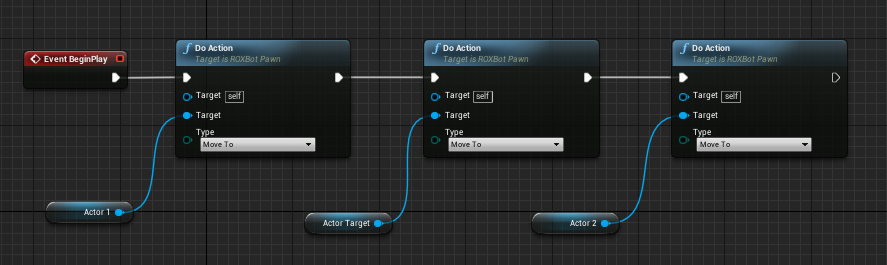
\includegraphics[scale=0.4]{archivos/action_queue.png}
	\centering
	\caption{Example of queuing 3 "MoveTo" actions from the editor}
	\label{action_queue}
\end{figure}

The $doAction()$ method creates a $FROXActions$ and pushes it to the queue. Whenever the queue contains an action and the $Pawn$ is not executing one, it will run the $fetchNextAction()$ method. This will pop the action from the queue and execute the method corresponding to that action.

Additionally, pathfinding and movement logic was implemented in order to define the $MoveTo$ action. In a first approach, the MoveToLocation method of the default \gls{ue4} Actor class was used, but the idea was discarded since we needed to work with the ROXBasePawn instead of the default Actor. Another option that was studied was Environment Query Systems (EQS), which is an experimental feature within the \gls{ai} system in \gls{ue4} and allows to gather data from the environment. It was finally discarded since the complexity of the technology was greater than that of the task we needed to solve, this is due to the fact that we only need the position of a certain actor in order to travel towards them, and this can be achieved without the need of more complex objects. 

With the previous options discarded, we decided to go with a custom implementation of the movement. In order to accomplish this, the NavigationMesh component of \gls{ue4} was used along with the $FindPathToActorSynchronously$ method, which returns a $UNavigationPath$ containing all the path-points from one actor to another. Once we obtain the path-points the $VInterpConstantTo$ from the FMath library and the $RInterpTo\_Constant$ from the UKismeMathLibrary are used in order to obtain the next vector transformation for both position and rotation of the $Pawn$, this movement logic can be seen in listing \ref{code:movementLogic}. These methods interpolate the current location with the next path-point location in order to achieve a smooth transition and make the movement more natural.

\begin{listing}[language=C++, caption=Movement logic for the pathfinding algorithm, frame=single, label=code:movementLogic]
	FVector nextPos = FMath::VInterpConstantTo(this->ActorLocation(), FVector(pathPoints[i].X, pathPoints[i].Y, ActorLocation().Z), DeltaTime, vel);
	FRotator nextRot = UKismetMathLibrary::RInterpTo_Constant(ActorRotation(), UKismetMathLibrary::FindLookAtRotation(ActorLocation(), nextPos), DeltaTime, rotateVel);
	SetActorRotation(nextRot);
	SetActorLocation(nextPos);
\end{listing}

\subsection{Animating the ROXBotPawn}
As we previously mentioned in section \ref{sec:sim2real}, simulating the 3D environment with extreme detail is a must in order for the algorithms to properly infer the knowledge and transfer it to the real world. In this section we will take a look into the process of creating a new animation for the ROXBotPawn using \gls{ue4} blueprints.

The ROXBasePawn already provides a default walking animation for our Actor, however it is thought to work with a VR Headset, therefore, it takes into account the pose and movement of both hand controllers and the headset itself in order to move accordingly to the user. Since our ROXBotPawn does not require such data, we will change the blueprint animation in order to fit our needs. 

First of all, we need the assets, in our case we will be using the default walk and idle animation from the UnrealROX framework. In order to have smooth transitions between different animations i.e from idle to walking, we have used \gls{ue4} BlendSpaces, which are special assets that can be sampled in the Animation Graph and allow for blended transitions based on one or more inputs. In our case,  we will blend the animation based on the speed of the Bot, a preview of said asset can be seen in Figure \ref{fig:blend_space}.

\begin{figure}[h]
	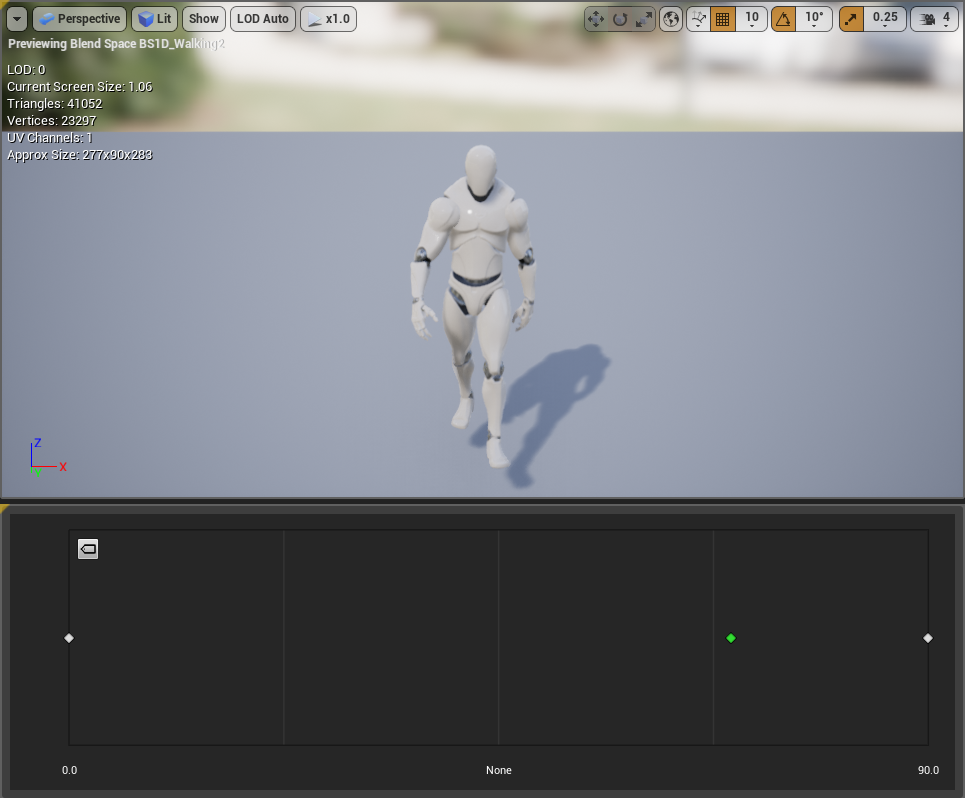
\includegraphics[width=0.5\textwidth]{archivos/blend_space.png}
	\centering
	\caption{Blend Space asset which samples the transition from idle walking state animation, 0 speed would translate into a complete idle, while 90 would be walking forward.}
	\label{fig:blend_space}
\end{figure}

In order to use the BlendSpaces, we need to create our Event Graph and compute the Bot speed, we do this by obtaining its position in the current and last tick, therefore obtaining the travel distance in one tick. We can now apply the dot operator with the forward vector and divide by the delta time, obtaining the current speed, the complete logic of this function as well as the full Event Graph can be seen in Figures \ref{fig:event_graph} and \ref{fig:speed_calc}.

\begin{figure}[h]
	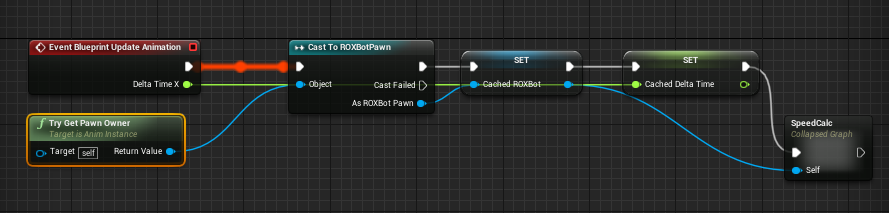
\includegraphics[width=\textwidth]{archivos/animation_event_graph.png}
	\centering
	\caption{Animation event graph which will obtain the Bot data, the SpeedCalc module is expanded in Figure \ref{fig:speed_calc}.}
	\label{fig:event_graph}
\end{figure}

\begin{figure}[h]
	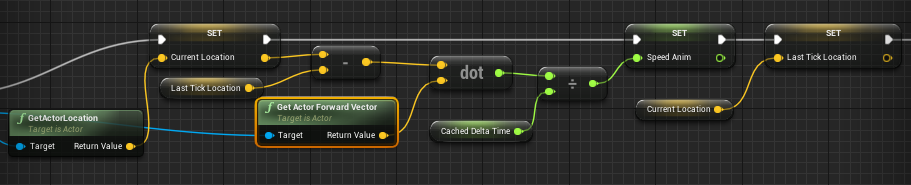
\includegraphics[width=\textwidth]{archivos/speed_calc.png}
	\centering
	\caption{Blueprint sub-module which computes the instantaneous speed of the Bot.}
	\label{fig:speed_calc}
\end{figure}

With the event graph and the BlendSpaces created all that is left to do is create the state machine which will contain the state and transition logic of the different animations. In our case, we just need an idle, walk forward and walk backwards states, this state machine is shown in Figure \ref{fig:state_machine}.

\begin{figure}[h]
	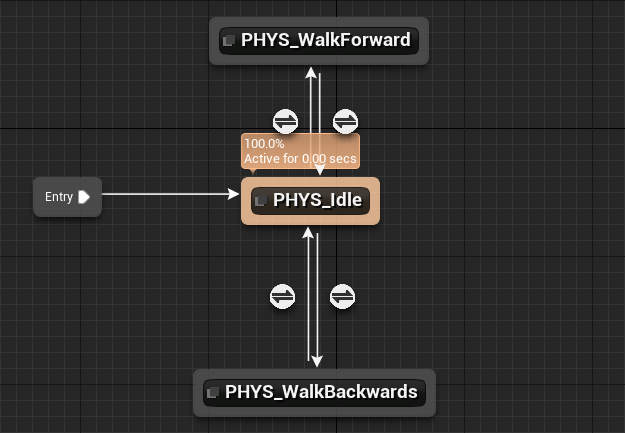
\includegraphics[scale=0.6]{archivos/animation_state_machine.png}
	\centering
	\caption{Animation state machine with idle, walk forward and walk backwards states and the transitions logic.}
	\label{fig:state_machine}
\end{figure}

The logic for the transitions between states are very simple, we will simply check if the speed surpasses a certain threshold, for instance, if the $Speed Anim$ is greater than 0.1, we will transition from the $Idle$ state to the $WalkForward$, in the same manner, when the speed value falls under negative $0.1$, we will transition towards the $WalkBackwards$ state.

\section{Recording sequences with UnrealROX}
\label{sec:tracker}
In the previous section, we developed the process of automatization of the framework in order to record sequences without the need of manually doing the actions with a VR Headset. In this section we will go through the ROXTracker class and how to use it in order to record sequences (subsection \ref{sec:recording}) as well as how to play them and generate the data (subsection \ref{sec:playback}).

The ROXTracker is an empty actor that has knowledge of the whole scene. In order to use it, we just need to search for it in the contextual menu (as shown in Figure \ref{fig:tracker_object}) and drag it to our scene. While in record mode, the ROXTracker will be able to store all of the information needed in order to rebuild the sequence offline as a TXT or JSON file, this will allow then to run the sequence in playback mode and generate frame by frame, ground truth annotated images such as the segmentation masks, depth and normal maps, as well as the RGB images.

\begin{figure}[h]
	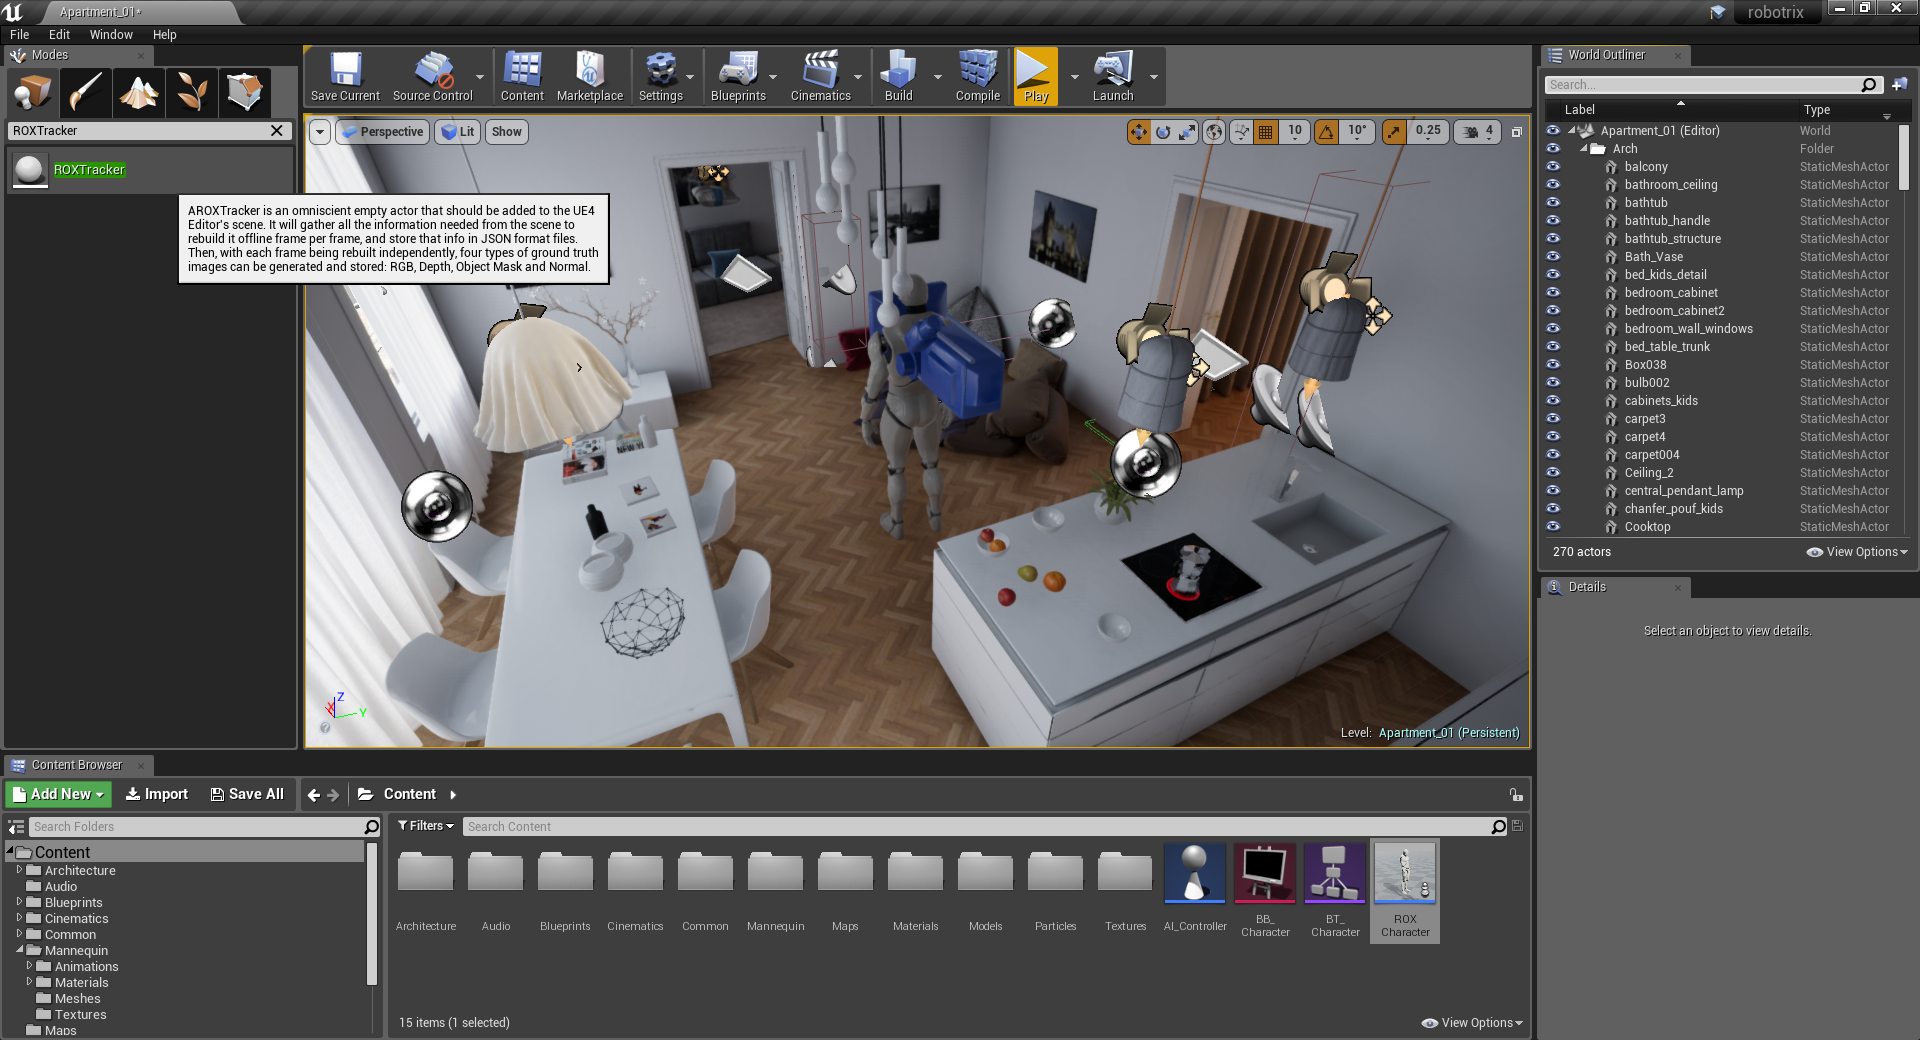
\includegraphics[width=\textwidth]{archivos/tracker_object.png}
	\centering
	\caption{ROXTracker Object in the \gls{ue4} contextual menu.}
	\label{fig:tracker_object}
\end{figure}

Once we have our ROXTracker in the World Outliner, we can tweak its behavior and change certain settings, some of the most important ones are listed as follows:

\begin{itemize}
	\item \textbf{Record Mode:} When checked, the ROXTracker will operate in record mode, this means that if the user presses the record key, it will start gathering and writing all of the necessary data to a TXT file.
	\item \textbf{Scene Save Directory:} As its own name implies, this variable stores the path where the data will be saved.
	\item \textbf{Scene Folder:}  Name of the folder inside the Scene Save Directory path where all the data files will be stored.
	\item \textbf{Generate Sequence Json:} When pressed will look for a TXT file inside the Secene Folder with name corresponding to the field \textbf{Input Scene TXT File Name} and will generate its equivalent JSON file with the name on the field \textbf{Output Scene Json File Name} i.e looking at Figure \ref{fig:tracker_settings}, the Tracker will search for a $scene.txt$ file inside the $unrealrox/RecordedSequences$ folder and generate a $scene.json$ file.
\end{itemize}

\begin{figure}[h]
	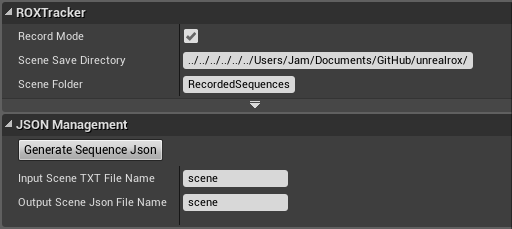
\includegraphics[width=0.8\textwidth]{archivos/tracker_settings.png}
	\centering
	\caption{ROXTracker settings in the \gls{ue4} editor.}
	\label{fig:tracker_settings}
\end{figure}

\subsection{Recording mode}
\label{sec:recording}

Before start generating sequences we have to make some tweaks to the recording settings of the ROXTracker, which can be seen in Figure \ref{fig:recording_settings} and further explained as follows:

\begin{itemize}
	\item \textbf{Pawns:} Array that contains a reference to every actor that the user wants to keep track of.
	\item \textbf{Camera Actors:} Array containing the cameras that will be tracked.
	\item \textbf{Stereo Camera Baselines:} Array that stores the focal distance (baseline) between the corresponding camera in the \textbf{CameraActors} array. It can be left empty if there are none.
	\item \textbf{Scene File Name Prefix:} Every generated file of raw scene data will share this prefix in its filename.
\end{itemize}

\begin{figure}[h]
	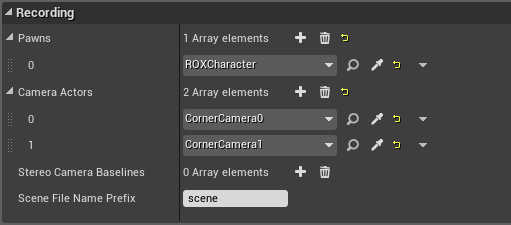
\includegraphics[width=0.5\textwidth]{archivos/recording_settings.png}
	\centering
	\caption{ROXTracker recording settings.}
	\label{fig:recording_settings}
\end{figure}

Once all of the fields are filled with the desired actors and cameras to be tracked and the filenames are set we can start recording a sequence, to do this, we simply have to set the ROXTracker in record mode and run the scene by hitting play on the editor. To begin/stop recording the user needs press "R", a red \textbf{RECORDING} message will display at the top of the screen, an example of the recorder running can be seen inf Figure \ref{fig:recording}.

\begin{figure}[h]
	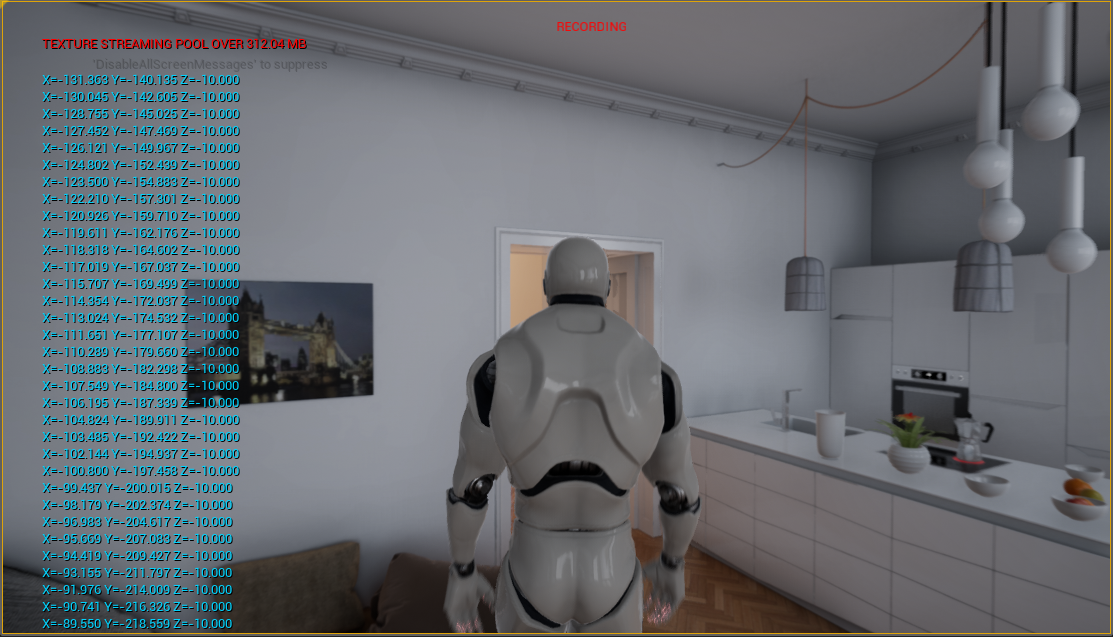
\includegraphics[width=0.6\textwidth]{archivos/recording.png}
	\centering
	\caption{Example of a running scene being recorded.}
	\label{fig:recording}
\end{figure}

When the sequence finishes, we can stop recording. If we take a look at our designated Scene Folder for the data generation we can se our recording raw data in TXT format. We now need, in order to get it ready for playback, parse it to JSON, we can do this with the \textbf{Generate Sequence Json} utility we have seen in Figure \ref{fig:tracker_settings}.

\subsection{Playback mode}
\label{sec:playback}

With our recording data in JSON format we are now able to play the sequences in the \gls{ue4} editor, but first we will go through some of the configuration settings for the playback mode, they can be seen in Figure \ref{fig:playback_settings} and are further explained below:

\begin{itemize}
	\item \textbf{Json File Names:} Array containing all the JSON filenames that we want to playback.
	\item \textbf{Start Frames:} Array that contains the starting frames for each JSON. The index in this array will directly correlate to the one in the \textbf{Json File Names} array.
	\item \textbf{Playback Only:} When active, it will only play the sequence, skipping the data generation process.
	\item \textbf{Playback Speed Rate:} As its own name indicates, allows to set the speed of the playback, although it can only be used in \textbf{Playback Only} mode. 
	\item \textbf{Generate RGB, Depth, Object Mask, Normal:} It will generate the RGB (format can be adjusted in the \textbf{Format RGB} option), Depth, Segmentation Masks and Normal maps for each frame and camera.
	\item \textbf{Generate Depth Txt Cm:} Generates an equivalent TXT file to the Depth image, where the depth values are stored as plain text.
	\item \textbf{Screenshot Save Directory:} Base path where the Screenshot folder will be located.
	\item \textbf{Screenshot Folder:} Name of the screenshot folder.
	\item \textbf{Width/Height:} Output resolution for the generated images.
\end{itemize}

\begin{figure}[h]
	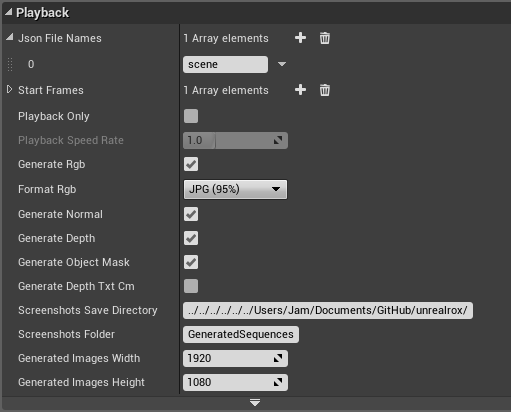
\includegraphics[width=0.5\textwidth]{archivos/playback_settings.png}
	\centering
	\caption{ROXTracker playback settings.}
	\label{fig:playback_settings}
\end{figure}

Once the desired configuration is set and the Record Mode is disabled , we can hit play in the editor. The ROXTracker object will start parsing the sequence JSON file and generating the output images in our designated folder, an example of the four different outputs is shown in Figure \ref{fig:playback_output}.

\begin{figure*}
	\centering
	\begin{subfigure}[b]{0.475\textwidth}
		\centering
		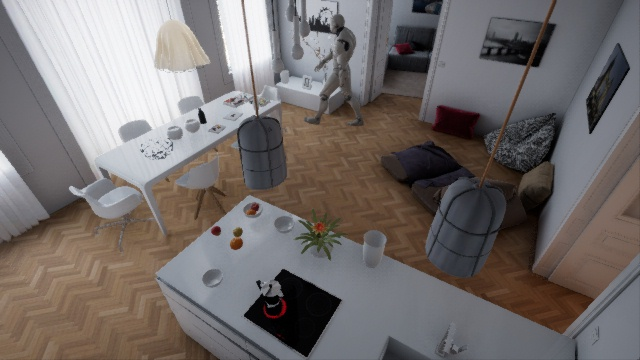
\includegraphics[width=\textwidth]{archivos/generated_rgb.jpg}
		\caption[Output RGB image.]%
		{{\small Output RGB image.}}    
		\label{fig:generated_rgb}
	\end{subfigure}
	\hfill
	\begin{subfigure}[b]{0.475\textwidth}  
		\centering 
		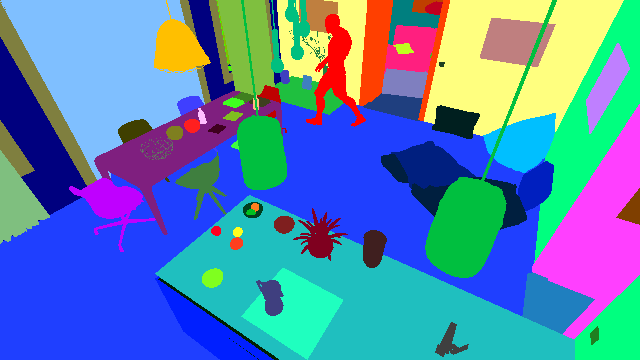
\includegraphics[width=\textwidth]{archivos/generated_mask.png}
		\caption[Output Segmentation Masks.]%
		{{\small Output Segmentation Masks.}}    
		\label{fig:generated_mask}
	\end{subfigure}
	\vskip\baselineskip
	\begin{subfigure}[b]{0.475\textwidth}   
		\centering 
		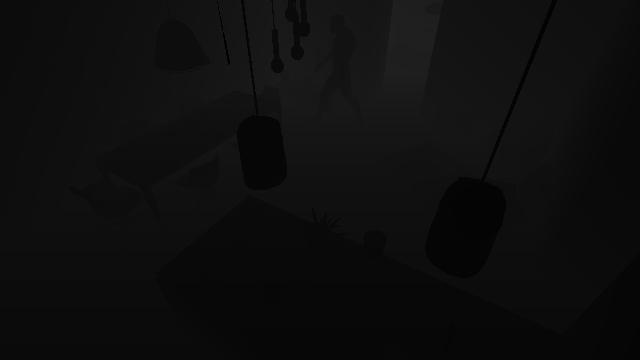
\includegraphics[width=\textwidth]{archivos/generated_depth.png}
		\caption[Output Depth image.]%
		{{\small Output Depth image.}}    
		\label{fig:generated_depth}
	\end{subfigure}
	\quad
	\begin{subfigure}[b]{0.475\textwidth}   
		\centering 
		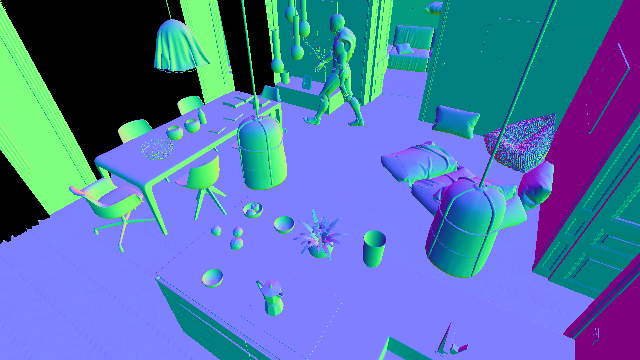
\includegraphics[width=\textwidth]{archivos/generated_normals.png}
		\caption[Output Normals image.]%
		{{\small Output Normals image.}}    
		\label{fig:generated_normals}
	\end{subfigure}
	\caption{Output examples of the Tracker in playback mode.}
	\label{fig:playback_output}
\end{figure*}

\section{Implementing a SegNet using PyTorch}
\label{sec:segnet}
As we previously mentioned, one of the main goals of this work is to study how synthetic data can help semantic segmentation algorithms. For this purpose, a SegNet has been implemented and trained with a real-world human-pose dataset, this section will cover the design and development process of such implementation.

\subsection{Preprocessing the dataset}
\label{sec:preprocess}
In section \ref{sec:datasets} we mentioned a few of the most important datasets in the field, however, all of them are general purpose oriented, and for this work we needed a human pose dataset. Because of this, we decided to use the Unite The People \cite{} dataset. Most of the images from this dataset come from the MPII Human Pose Dataset and contains both the RGB and the Segmentation Mask image.

However, some data pre-processing will be needed in order to fit the dataset to our needs.

\subsubsection{Merging the segmentation masks}

\subsubsection{Creating the dataset class} 

\subsection{Training the network}
\label{sec:training}

\subsubsection{SegNet Model}

\subsubsection{Training script}
